\section{programme parallèle MPI}

La courbe de la figure \ref{fig:perf_plumer2048bare2048_MPI} représente les résultats obtenus après l'exécution de notre programme sur les corps du fichier baredisk\_2048-plummer\_2048.nemo avec MPI seulement.

\par D'après ce graphe, on constate que les calculs en utilisant un processus MPI par coeur sont un peu plus rapides. En effet, les machines utilisées pour effectuer les mesures sont équipées d'un processeur ``Quad Core''. Lancer 4 processus MPI sur une seule machine est équivalent à lancer un processus MPI sur chaque coeur de cette machine. Or, les communications sont relativement ``négligeables'' lorsque l'on travaille sur la même machine, ce qui explique le temps qu'on gagne (voir \ref{fig:perf_plumer2048bare2048_MPI}) tout au début de la mesure avec 4 processus MPI.

\par Pour le reste des cas, les temps d'exécution des calculs avec les deux méthodes, d'un coté, celle utilisant un processus MPI par machine et de l'autre, celle utilisant un processus MPI par coeur, restent relativement identiques.

\begin{figure}[htbp]
  \centering
  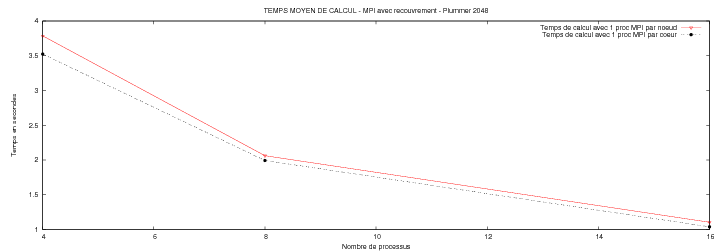
\includegraphics[angle=90]{perf_plumer2048bare2048_MPI.png}
  \caption{Temps total de calcul avec MPI}
  \label{fig:perf_plumer2048bare2048_MPI}
\end{figure}

\section{programme parallèle hybride MPI+OPEN\_MP}
La courbe de la figure \ref{fig:perf_plumer2048bare2048} représente les résultats obtenus après l'exécution de notre programme sur les corps du fichier baredisk\_2048-plummer\_2048.nemo avec MPI-openMP.

\begin{figure}[htbp]
  \centering
  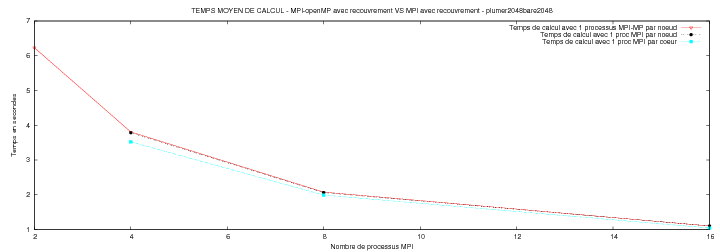
\includegraphics[angle=90]{perf_plumer2048bare2048.png}
 \caption{Temps total de calcul avec MPI couplé avec openMP}
\label{fig:perf_plumer2048bare2048}
\end{figure}
